
\subsection{Res}


\setlength{\arrayrulewidth}{1mm}
\setlength{\tabcolsep}{18pt}
\renewcommand{\arraystretch}{2.5}

\begin{tabular}{ |p{3cm}||p{3cm}|p{3cm}|p{3cm}|  }
 \hline
 \multicolumn{4}{|c|}{Country List} \\
 \hline
 Country Name     or Area Name& ISO ALPHA 2 Code &ISO ALPHA 3 Code&ISO numeric Code\\
 \hline
 Afghanistan   & AF    &AFG&   004\\
 Aland Islands&   AX  & ALA   &248\\
 Albania &AL & ALB&  008\\
 Algeria    &DZ & DZA&  012\\
 American Samoa&   AS  & ASM&016\\
 Andorra& AD  & AND   &020\\
 Angola& AO  & AGO&024\\
 \hline
\end{tabular}

\begin{verbatim}[commandchars=\\\{\}]
   RheobaseTest  InputResistanceTest  TimeConstantTest  CapacitanceTest  \textbackslash{}
      1.133177             0.444622          0.450915         0.029973

   RestingPotentialTest  InjectedCurrentAPWidthTest  \textbackslash{}
              0.012897                     0.16468

   InjectedCurrentAPAmplitudeTest  InjectedCurrentAPThresholdTest
                       0.003763                        0.512854
\end{verbatim}

\begin{verbatim}[commandchars=\\\{\}]
   chi\_square   p\_value
    2.125091  0.976935
\end{verbatim}

%\begin{tcolorbox}[breakable, size=fbox, boxrule=.5pt, pad at break*=1mm, opacityfill=0]
\begin{verbatim}[commandchars=\\\{\}]
   RheobaseTest  InputResistanceTest  TimeConstantTest  CapacitanceTest  \textbackslash{}
      0.536865             0.100485          0.717214         0.133624

   RestingPotentialTest  InjectedCurrentAPWidthTest  \textbackslash{}
              0.055446                     0.16846

   InjectedCurrentAPAmplitudeTest  InjectedCurrentAPThresholdTest
                        0.039952                        1.123152
\end{verbatim}

    

\begin{center}
   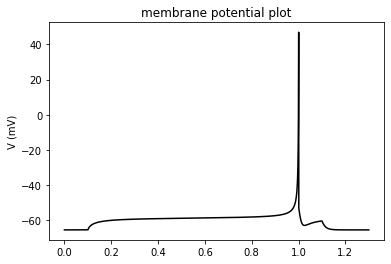
\includegraphics[width=0.7\linewidth]{notebooks_converted/make_normal_distribution_files/make_normal_distribution_8_2}
\end{center}
{ \hspace*{\fill} \\}

            
    \begin{verbatim}[commandchars=\\\{\}]
       chi\_square   p\_value
       17.216463  0.027932
    \end{verbatim}

\begin{verbatim}[commandchars=\\\{\}]
   chi\_square   p\_value
   17.216463  0.027932
\end{verbatim}

\begin{verbatim}[commandchars=\\\{\}]
   RheobaseTest  InputResistanceTest  TimeConstantTest  CapacitanceTest  \textbackslash{}
      0.104364              0.26776          0.909698         0.779279

   RestingPotentialTest  InjectedCurrentAPWidthTest  \textbackslash{}
              0.263258                    2.539904

   InjectedCurrentAPAmplitudeTest  InjectedCurrentAPThresholdTest                        0.197484                        3.023183
\end{verbatim}

\begin{center}
    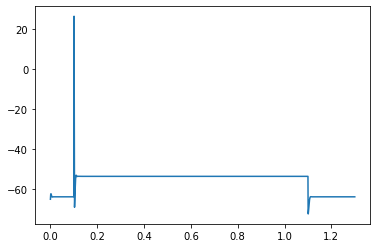
\includegraphics[width=0.7\linewidth]{notebooks_converted/make_normal_distribution_files/make_normal_distribution_15_0}
\end{center}

\begin{verbatim}[commandchars=\\\{\}]
                    
chi\_square  10.232514
p\_value      0.249084
\end{verbatim}

\begin{verbatim}[commandchars=\\\{\}]
   RheobaseTest  InputResistanceTest  TimeConstantTest  CapacitanceTest  \textbackslash{}
      0.173923             0.512072          0.865851         0.319662

   RestingPotentialTest  InjectedCurrentAPWidthTest  \textbackslash{}
              0.140107                    2.952786

   InjectedCurrentAPAmplitudeTest  InjectedCurrentAPThresholdTest
                        0.318337                        0.498246
\end{verbatim}

\begin{verbatim}[commandchars=\\\{\}]
                   0
chi\_square  2.019044
p\_value     0.980422
\end{Verbatim}
\end{tcolorbox}
        
\begin{tcolorbox}[breakable, size=fbox, boxrule=.5pt, pad at break*=1mm, opacityfill=0]
\begin{Verbatim}[commandchars=\\\{\}]
   InputResistanceTest  TimeConstantTest  CapacitanceTest  \textbackslash{}
             0.209574          0.178053         0.030453

   RestingPotentialTest  InjectedCurrentAPWidthTest  \textbackslash{}
              0.297853                     0.19034

   InjectedCurrentAPAmplitudeTest  InjectedCurrentAPThresholdTest
                        0.035634                        1.347693
\end{verbatim}

